% Standalone source for fig_architecture.pdf
% Compile:  pdflatex fig_architecture.tex    (run inside paper/figures/)
\documentclass[border=2pt]{standalone}
\usepackage{tikz}
\usetikzlibrary{positioning,arrows.meta,fit,backgrounds}
\begin{document}
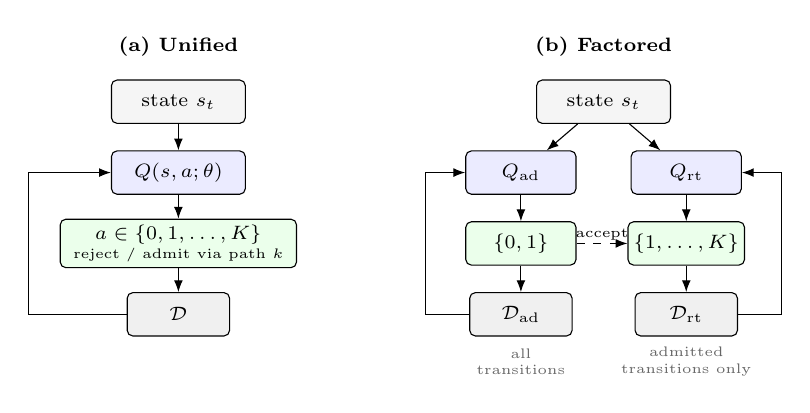
\begin{tikzpicture}[
  font=\scriptsize,
  box/.style={draw,rounded corners=2pt,minimum height=5.5mm,align=center,inner sep=2pt},
  net/.style={box,fill=blue!8,minimum width=17mm},
  act/.style={box,fill=green!8},
  buf/.style={box,fill=black!6,minimum width=13mm},
  >={Latex[length=1.5mm]}
]
% ---------------- unified ----------------
\node[align=center,font=\scriptsize\bfseries] at (0,1.55) {(a) Unified};
\node[box,fill=black!4,minimum width=17mm] (s1) at (0,0.85) {state $s_t$};
\node[net] (q1) at (0,-0.05) {$Q(s,a;\theta)$};
\node[act,minimum width=30mm] (a1) at (0,-0.95)
     {$a\in\{0,1,\dots,K\}$\\[-1pt]\tiny reject / admit via path $k$};
\node[buf] (d1) at (0,-1.85) {$\mathcal{D}$};
\draw[->] (s1)--(q1); \draw[->] (q1)--(a1); \draw[->] (a1)--(d1);
\draw[->] (d1.west) -- ++(-1.25,0) |- (q1.west);

% ---------------- factored ----------------
\begin{scope}[xshift=5.4cm]
\node[align=center,font=\scriptsize\bfseries] at (0,1.55) {(b) Factored};
\node[box,fill=black!4,minimum width=17mm] (s2) at (0,0.85) {state $s_t$};
\node[net,minimum width=14mm] (qa) at (-1.05,-0.05) {$Q_{\mathrm{ad}}$};
\node[net,minimum width=14mm] (qr) at (1.05,-0.05) {$Q_{\mathrm{rt}}$};
\node[act,minimum width=14mm] (aa) at (-1.05,-0.95) {$\{0,1\}$};
\node[act,minimum width=14mm] (ar) at (1.05,-0.95) {$\{1,\dots,K\}$};
\node[buf] (da) at (-1.05,-1.85) {$\mathcal{D}_{\mathrm{ad}}$};
\node[buf] (dr) at (1.05,-1.85) {$\mathcal{D}_{\mathrm{rt}}$};
\draw[->] (s2)--(qa); \draw[->] (s2)--(qr);
\draw[->] (qa)--(aa); \draw[->] (qr)--(ar);
\draw[->] (aa)--(da); \draw[->] (ar)--(dr);
\draw[->,dashed] (aa.east) -- node[above,font=\tiny,inner sep=1pt]{accept} (ar.west);
\draw[->] (da.west) -- ++(-0.55,0) |- (qa.west);
\draw[->] (dr.east) -- ++(0.55,0) |- (qr.east);
\node[font=\tiny,align=center,text=black!60] at (1.05,-2.45)
     {admitted\\transitions only};
\node[font=\tiny,align=center,text=black!60] at (-1.05,-2.45)
     {all\\transitions};
\end{scope}
\end{tikzpicture}
\end{document}
